\documentclass[9pt]{beamer}
\mode<presentation>
\usepackage[T1]{fontenc}
\usepackage{color}
\usepackage{graphicx}
\usepackage{natbib}
\usepackage{tikz}
\usetikzlibrary{shapes.geometric}
\usepackage{xmpmulti}
\usepackage{animate}
\usepackage{tcolorbox}
\usepackage{amsmath}
\usepackage{gensymb}
\usepackage{csquotes}

\usetheme{Singapore}
%\usecolortheme{seahorse}

\usefonttheme{professionalfonts}

\title[Word \& Doc Embeddings]{Machine Assisted Rapid Review}
\author{Max Callaghan, Finn Müller-Hansen}
\institute[MCC]{
	
\includegraphics[height=1cm,width=2cm]{../images/MCC_Logo_RZ_rgb.jpg}
}

\newif\ifframeinlbf
\frameinlbftrue
\makeatletter
\newcommand\listofframes{\@starttoc{lbf}}
\makeatother

\addtobeamertemplate{frametitle}{}{%
	\ifframeinlbf
	\addcontentsline{lbf}{section}{\protect\makebox[2em][l]{%
			\protect\usebeamercolor[fg]{structure}\insertframenumber\hfill}%
		\insertframetitle\par}%
	\else\fi
}

\newtheorem*{remark}{}

\bibliographystyle{apalike}

\begin{document}
	
\begin{frame}
	\titlepage
\end{frame}

\section{Introduction}

\begin{frame}{Screening}

In systematic review, we want to have a broad search query, to make sure we include as many relevant documents as possible

\bigskip

This means we need to screen all of the documents the search query returns, in order to find a clean set of relevant documents.


\end{frame}

\begin{frame}{Machine Assisted Screening}

\begin{itemize}

	\item Scientific literature is expanding in all subject areas, increasing the work needed to conduct systematic reviews.
	
	\item The process generates training data, making it an ideal setting for applying \textit{Active Learning} see \cite{Settles2009}
	
	\item An expanding literature exists on using active learning for screening in systematic reviews \cite{OMara-Eves2015}
	
\end{itemize}


\end{frame}

\section{Approach}

\begin{frame}{Active Learning} 

\begin{figure}
	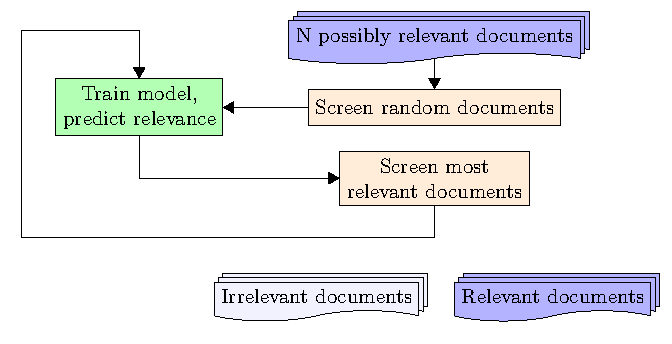
\includegraphics[width=0.8\linewidth]{../images/flow_basic.pdf}
\end{figure}

When do we stop? How can we describe when we stopped, and what we think this means about the literature we have selected and not selected?

$ Precision=1.0 $, but what about $Recall$?

\end{frame}

\begin{frame}{Missing stopping criteria}


Research on a Stopping criterion in AL literature suggest stopping when the confidence or performance of the classifier drops. These indicate when the ML part is no longer generating useful results, but do not relate to recall: Vlachos stress that ``the remaining instances should be considered redundant only for the given model and feature representation'' \cite{Vlachos2008}

\medskip
 
Stopping criteria in the systematic review literature are not well articulated:

\blockcquote{miwa2014}{Once a given stopping criterion is reached (for example, when all relevant studies have been identified, or when the reviewers have run out of time for manual screening), the process ceases, and the remainder of studies not yet screened manually is discarded}

\end{frame}

\begin{frame}{Missing stopping criteria}
Statistical approaches are hinted at but underdeveloped:


\blockcquote{Przybya2018}{Deciding when to stop can be left to the end-user, eg, if the prioritised references are consistently irrelevant, or heuristics or statistical approaches (based on an unbiased sample of the remaining references) can inform this decision. We intend to investigate this problem in the future}

\medskip

A reliable stopping criterion is still a research gap:

\blockcquote{bannach-brown2019}{The problem of choosing a cut-off threshold, equivalent to deciding when to stop when using a model for prioritising relevant documents, remains an open research question in information retrieval}

\end{frame}

\begin{frame}{Relevance of unseen documents is insufficient}
\begin{figure}
	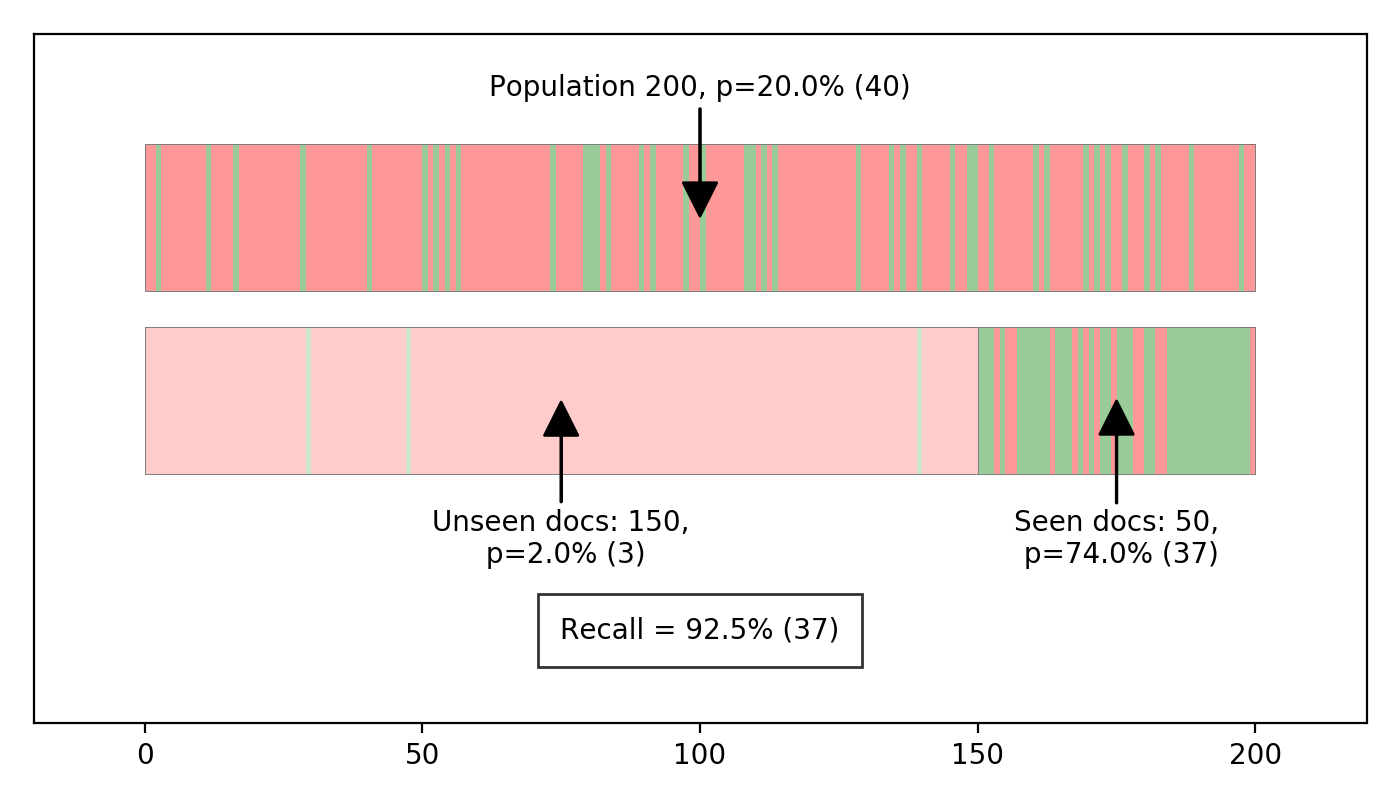
\includegraphics[width=\linewidth]{../images/proportions_1}<1>
	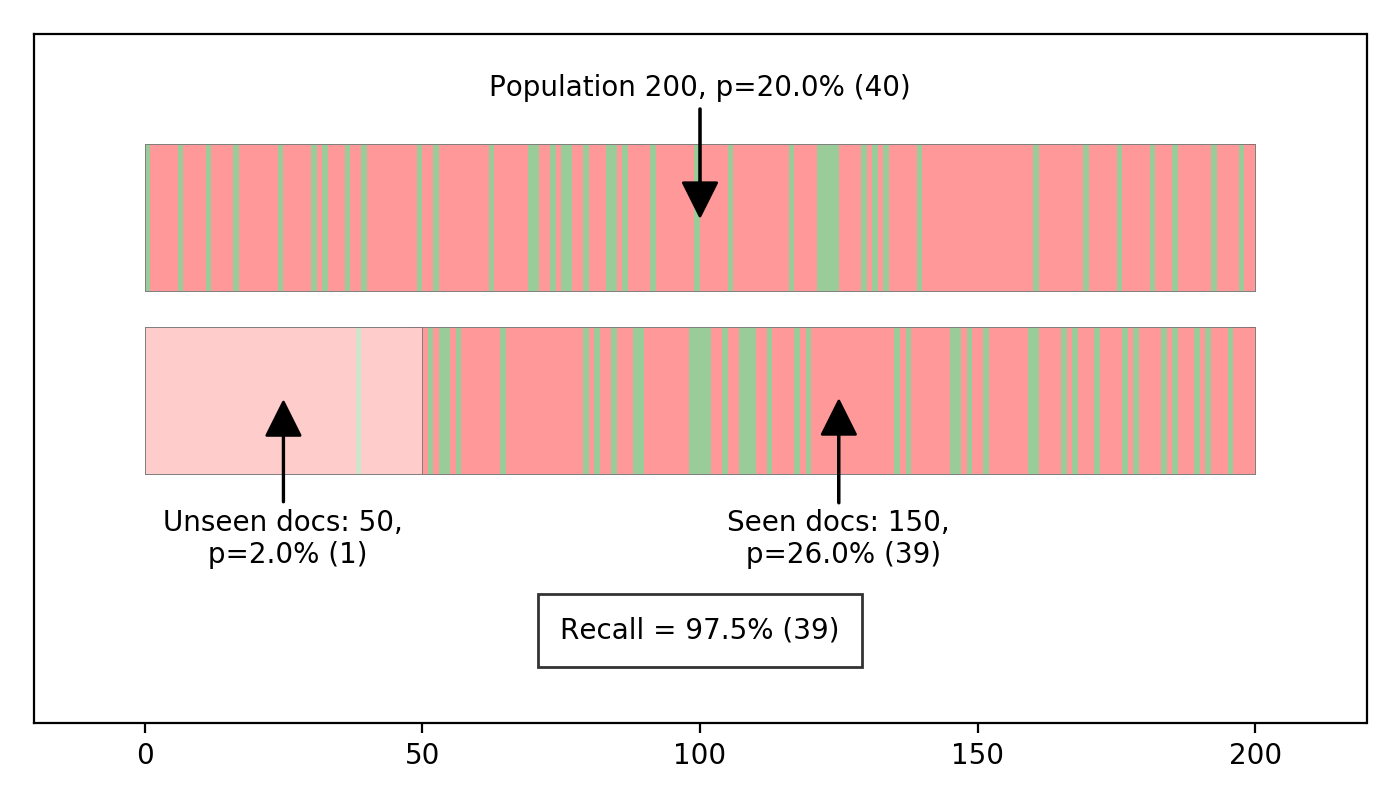
\includegraphics[width=\linewidth]{../images/proportions_2}<2>
\end{figure}
\end{frame}

\begin{frame}{Relevance of unseen documents is insufficient}
\begin{columns}
	\begin{column}{0.6\linewidth}
		\begin{figure}
			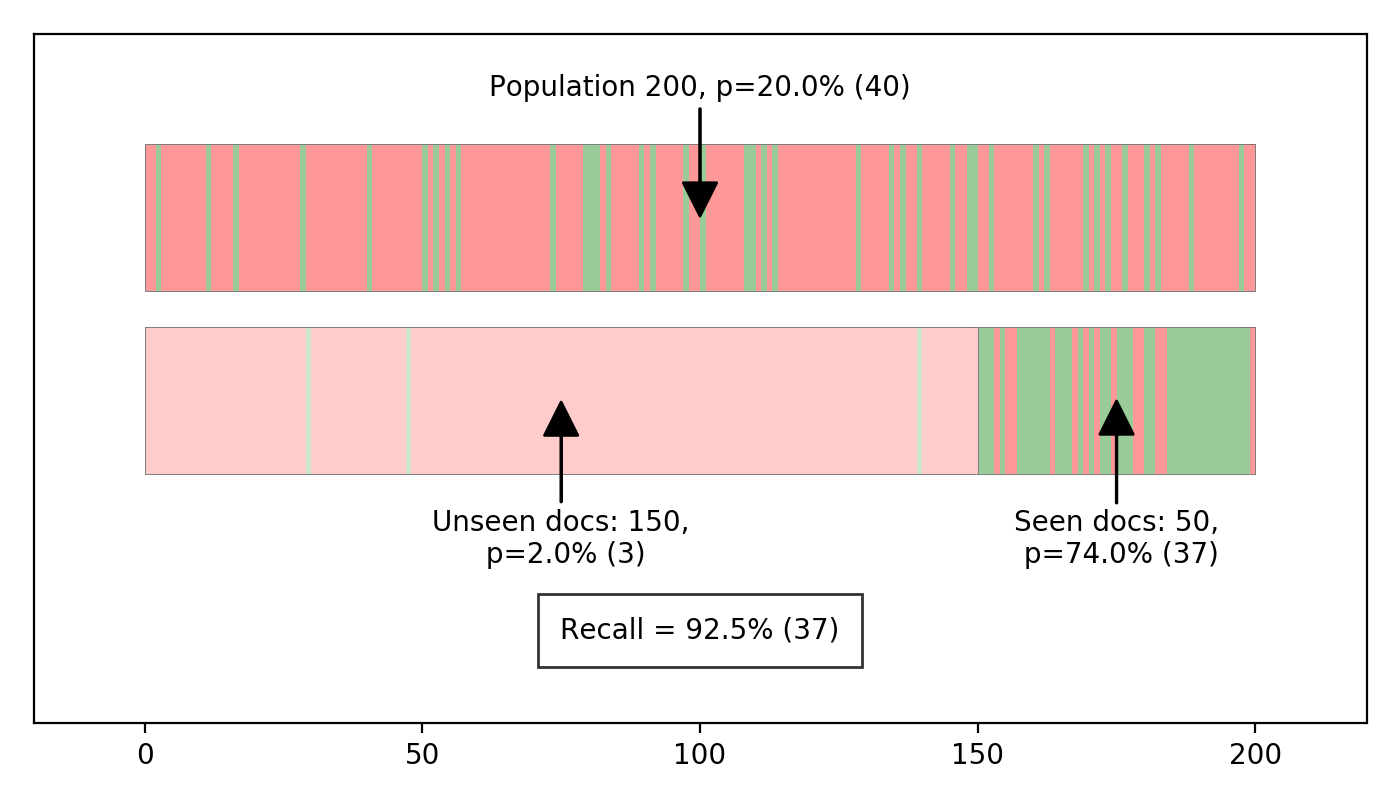
\includegraphics[width=\linewidth]{../images/proportions_1}
			
			\vspace{-1em}
			
			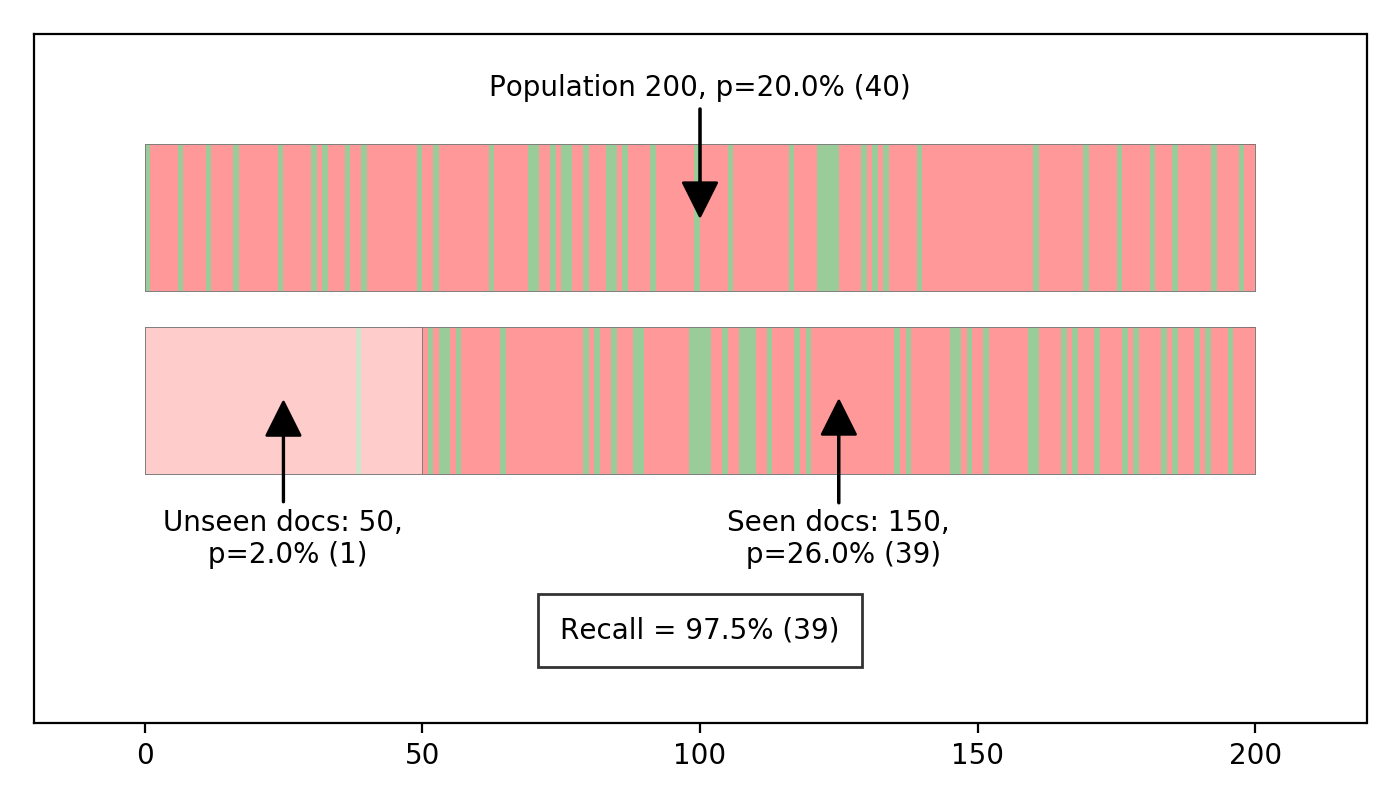
\includegraphics[width=\linewidth]{../images/proportions_2}
		\end{figure}
	\end{column}
	\begin{column}{0.4\linewidth}
			\only{It doesn't just matter what proportion of unseen documents is relevant, but also what proportion of documents is unseen
			}<1->
		
		\bigskip
		
		\only{We can calculate the recall with the relevance of the unseen docs, the relevance of the population and porportion of documents seen
			
			\[ 1 - \frac{pU}{pP} \frac{U}{P} \]
		
		}<2->
	\end{column}
\end{columns}

\end{frame}

\begin{frame}{Uncertainty of pU}

 However, without perfect knowledge, we don't \textit{know} the relevance of unseen documents: but we can \textit{estimate} it through taking a sample. We do know \(U\), the number of unseen documents, \(S\), the number of seen documents, and \( pS \), the relevance of seen documents, 
 
 \bigskip
\begin{tabular}{p{0.618\linewidth} p{0.382\linewidth}}
 For a given p-value, we can generate an Agresti-Coull interval & 
 \( CI_{AC} = \tilde{p} \pm \kappa(\tilde{p}\tilde{q})^{1/2}\tilde{n}^{-1/2} \) \\
  & \\
 We can use the outer limit \( \dot{p} = \max\tilde{p} \) to estimate the relevance of all documents 
  &  \( \dot{p}P = \frac{pS*S + \dot{p}U*U}{N}  \) \\
  & \\
 And plug both of these into the original equation to generate a minimum estimated recall & 
 \( \hat{R} = 1- \frac{\dot{p}U}{\dot{p}P} \frac{U}{P} \)
 
\end{tabular}

\bigskip

We can set the recall and confidence interval prior to the start of screening

\end{frame}

\begin{frame}{Uncertainty of pU}

\begin{columns}
	\begin{column}{0.5\linewidth}
		\begin{figure}
			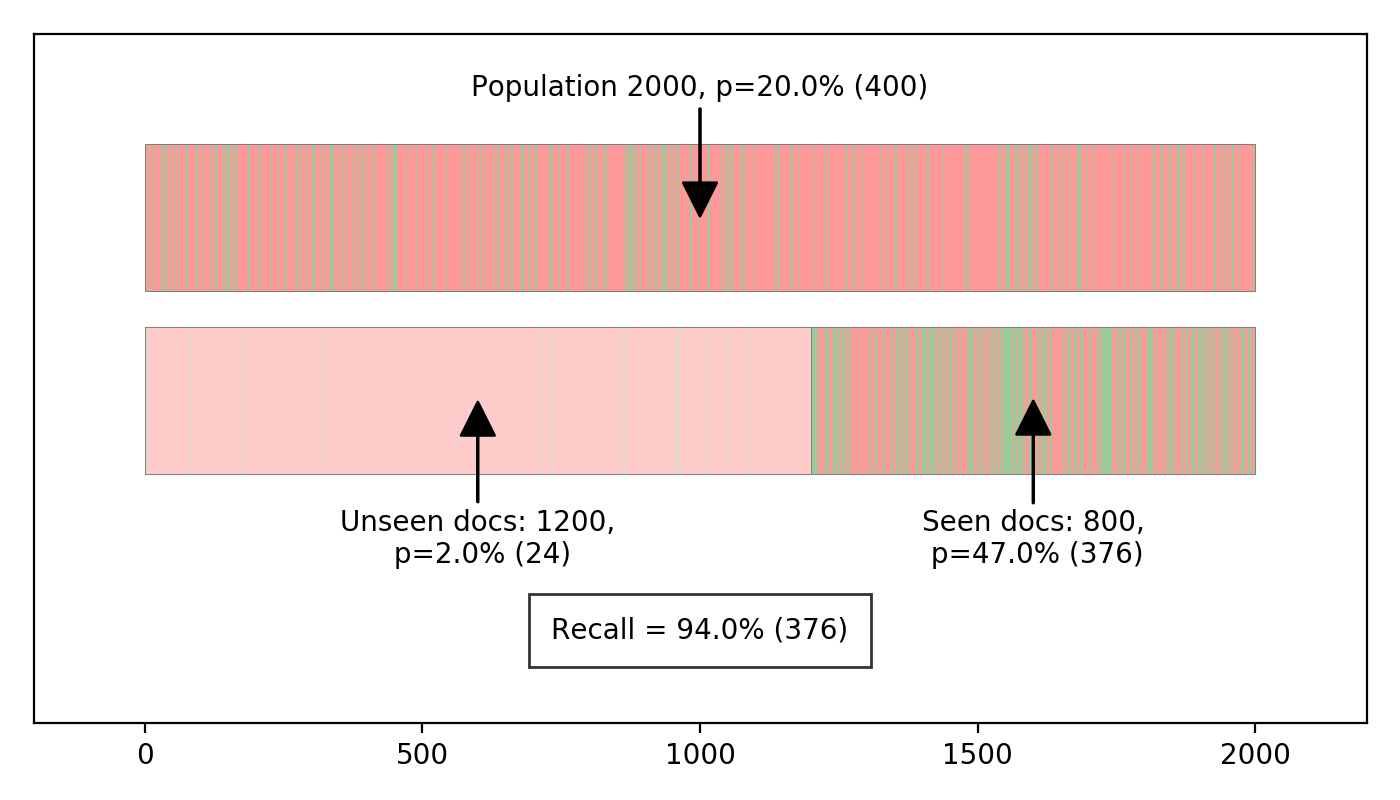
\includegraphics[width=\linewidth]{../images/sample_status.png}
		\end{figure}
	\end{column}
	\begin{column}{0.5\linewidth}
		\begin{figure}
			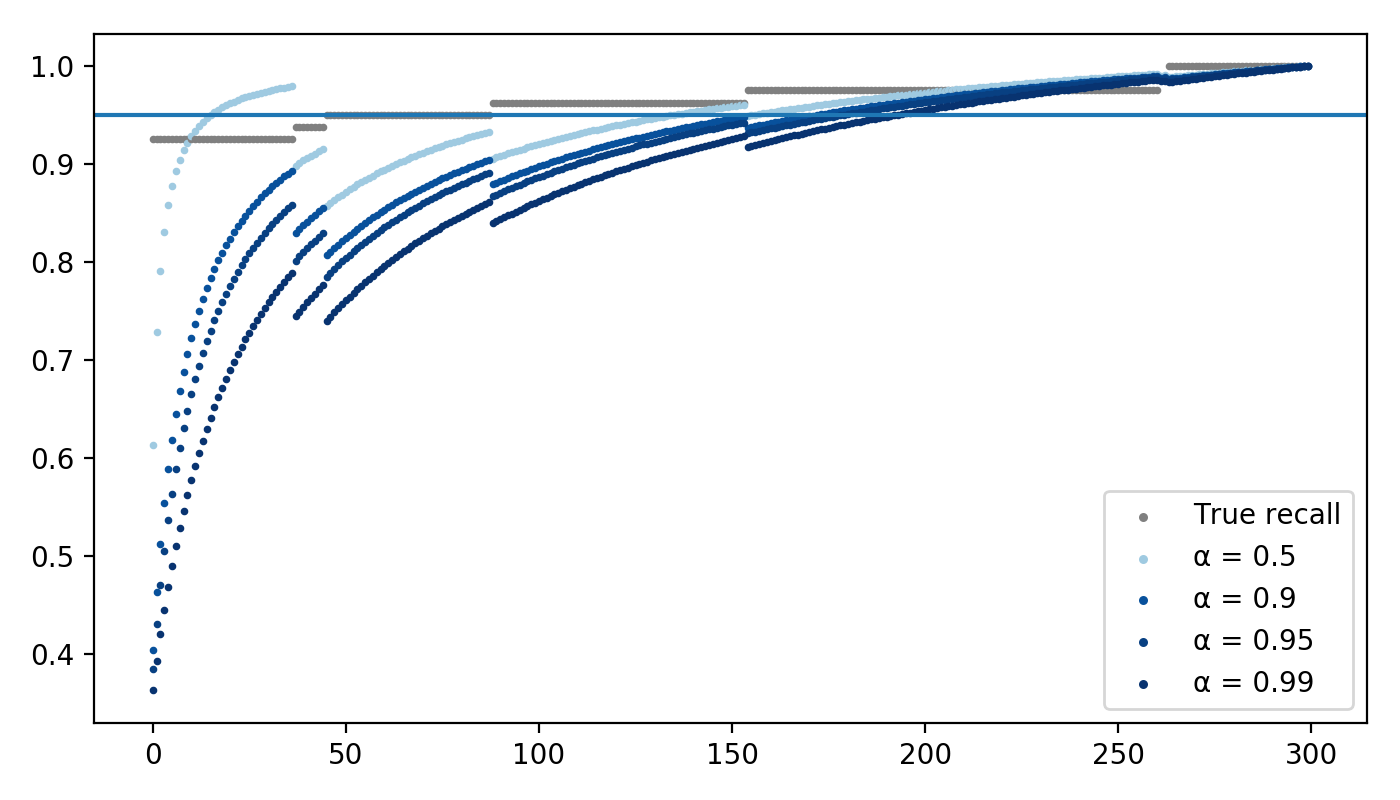
\includegraphics[width=\linewidth]{../images/sample_recall.png}
		\end{figure}
	\end{column}
\end{columns}

\end{frame}

\begin{frame}{Uncertainty of pU}

\begin{columns}
	\begin{column}{0.5\linewidth}
		\begin{figure}
			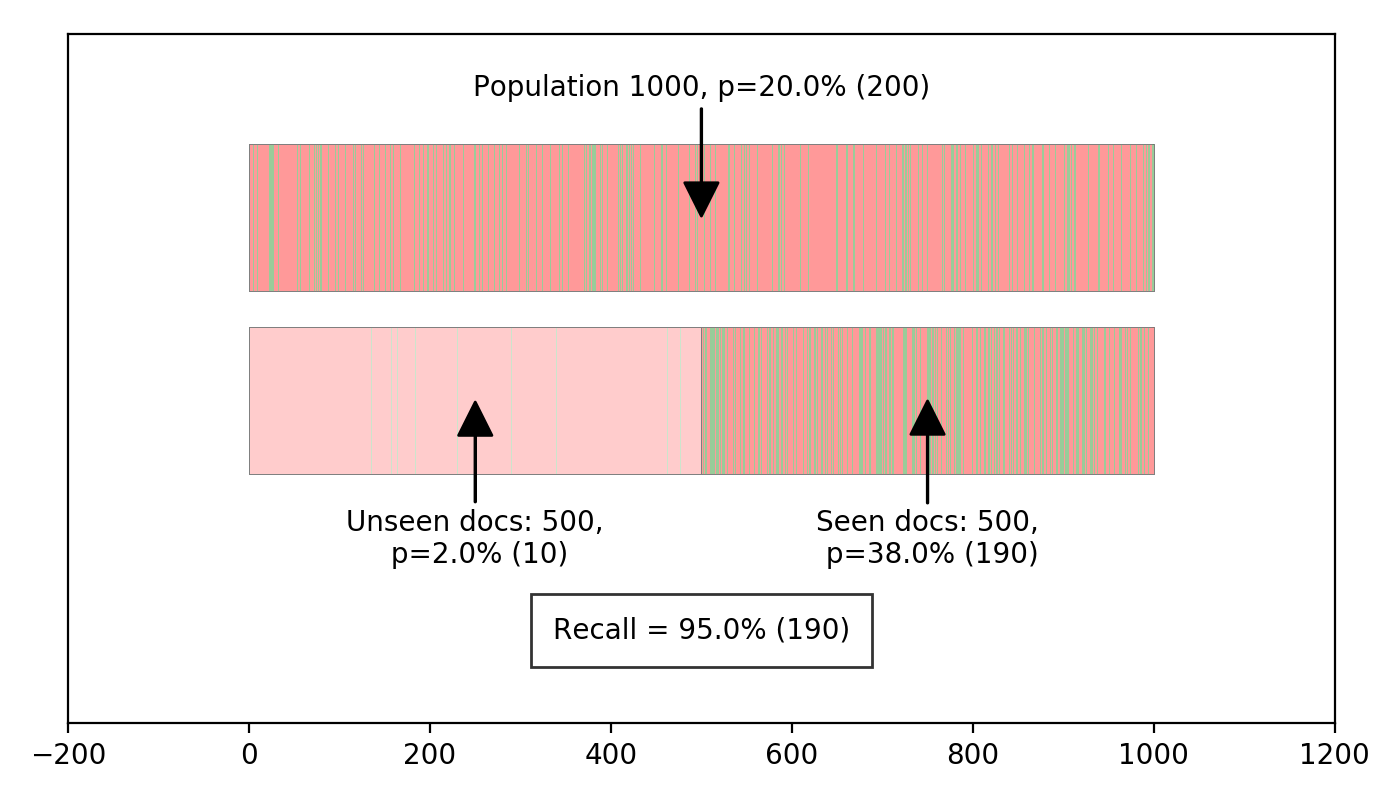
\includegraphics[width=\linewidth]{../images/sample_status_2.png}
		\end{figure}
	\end{column}
	\begin{column}{0.5\linewidth}
		\begin{figure}
			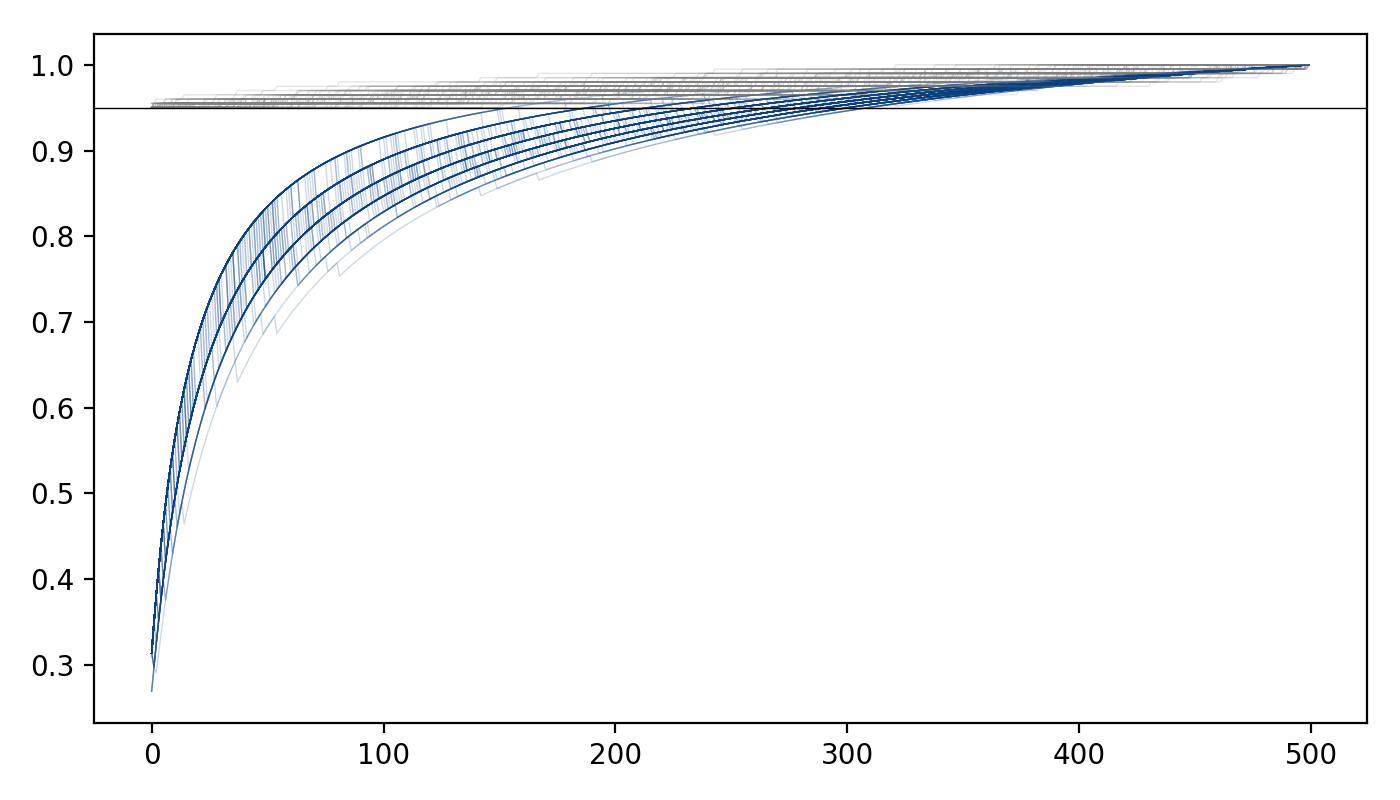
\includegraphics[width=\linewidth]{../images/sample_recall_2.png}
		\end{figure}
	\end{column}

\end{columns}

\bigskip

	\[   CI_{AC} = \tilde{p} \pm \kappa(\tilde{p}\tilde{q})^{1/2}\tilde{n}^{-1/2}  \]
	
\[ \hat{R} = 1- \frac{\dot{p}U}{\dot{p}P} \frac{U}{P} \]

\end{frame}

\begin{frame}{Active Learning with Robust Probabilistic Stopping Criteria} 

\begin{figure}
	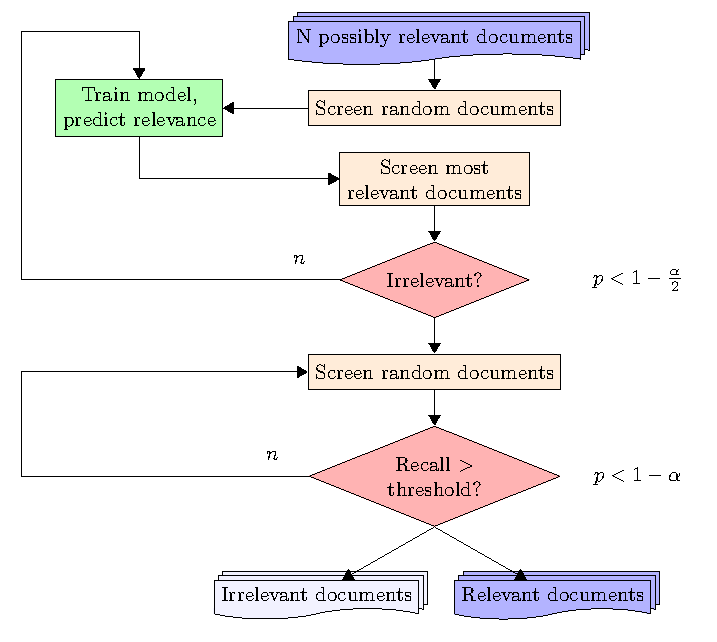
\includegraphics[width=0.8\linewidth]{../images/flow.pdf}
\end{figure}

\end{frame}

\section{Evaluation}

\begin{frame}{Evaluation on existing dataset(s)}
To be done - ours? Someone elses? Simulations with many types/specifications of ML models, showing reduction in work, predicted and actual recall

\bigskip

Necessary?
\end{frame}

\section{Question}

\begin{frame}{How big should the sample be?}

What confidence intervals do we get for different levels of relevance and different sample sizes?

\bigskip

Increasing N reduces unseen docs and size of confidence interval

\end{frame}

\begin{frame}{Do we need to take a sample?}

Could we just keep looking at the most relevant documents (this would make our estimates more conservative) or does this just make things complicated without saving time?

\end{frame}

\begin{frame}{When do we move from the most relevant documents to a random sample?}

Is this when we find no more relevant documents? When no more relevant documents are predicted? When model performance on new data drops below a certain level? Some other criterion or combination of criteria?

\end{frame}

\begin{frame}{Do we need to rate all documents in the sample?}

Can the system estimate recall as we rate documents, and stop as soon as we have reached the threshold?

\end{frame}

\begin{frame}{What if we prioritised irrelevant documents?}

In this way we could be certain about recall, and uncertain about precision.

\bigskip

We spend a lot of time looking at irrelevant documents (so learn less about the literature during the process), but sometimes exclusion decisions can be faster than inclusion decisions.

\end{frame}

\section{Conclusion}

\begin{frame}{Conclusion}

This is a new way to use machine learning in screening

\begin{itemize}
	\item<1-> Offers robust stopping criteria
	\item<2-> ML model performance does not determine accuracy of document selection, only influences work reduction
\end{itemize}

\end{frame}

\begin{frame}
\listofframes
\end{frame}

\begin{frame}{References}
\bibliography{../mendeley}
\end{frame}


\end{document}